\chapter{Rancangan}
\label{chap:rancangan}
Bab ini menjelaskan perancangan aplikasi, termasuk algoritma-algoritma untuk mengolah \textit{Google StreetView API}, \textit{Google Directions API}, serta modifikasi yang dilakukan pada aplikasi HelloVR untuk membangun aplikasi \textit{jogging} virtual. 


\section{Rancangan Antarmuka}
Aplikasi yang akan dibangun terdiri atas dua halaman utama, yaitu halaman utama dan halaman VR.

\subsection{Halaman Utama}
\label{subs:main-page}
Halaman utama adalah halaman yang ditampilkan pertama kali saat pengguna membuka aplikasi dengan \textit{portrait layout}. Fungsi halaman ini adalah menerima masukan pengguna, yaitu lokasi asal dan lokasi tujuan saat berlari, serta memicu halaman kedua, yaitu halaman VR. Ada tiga komponen utama dari halaman ini, yaitu dua buah \textit{textbox} dan sebuah tombol. Gambar \ref{fig:main-page} menggambarkan tampilan halaman utama.  

\begin{figure}[h]
	\centering
		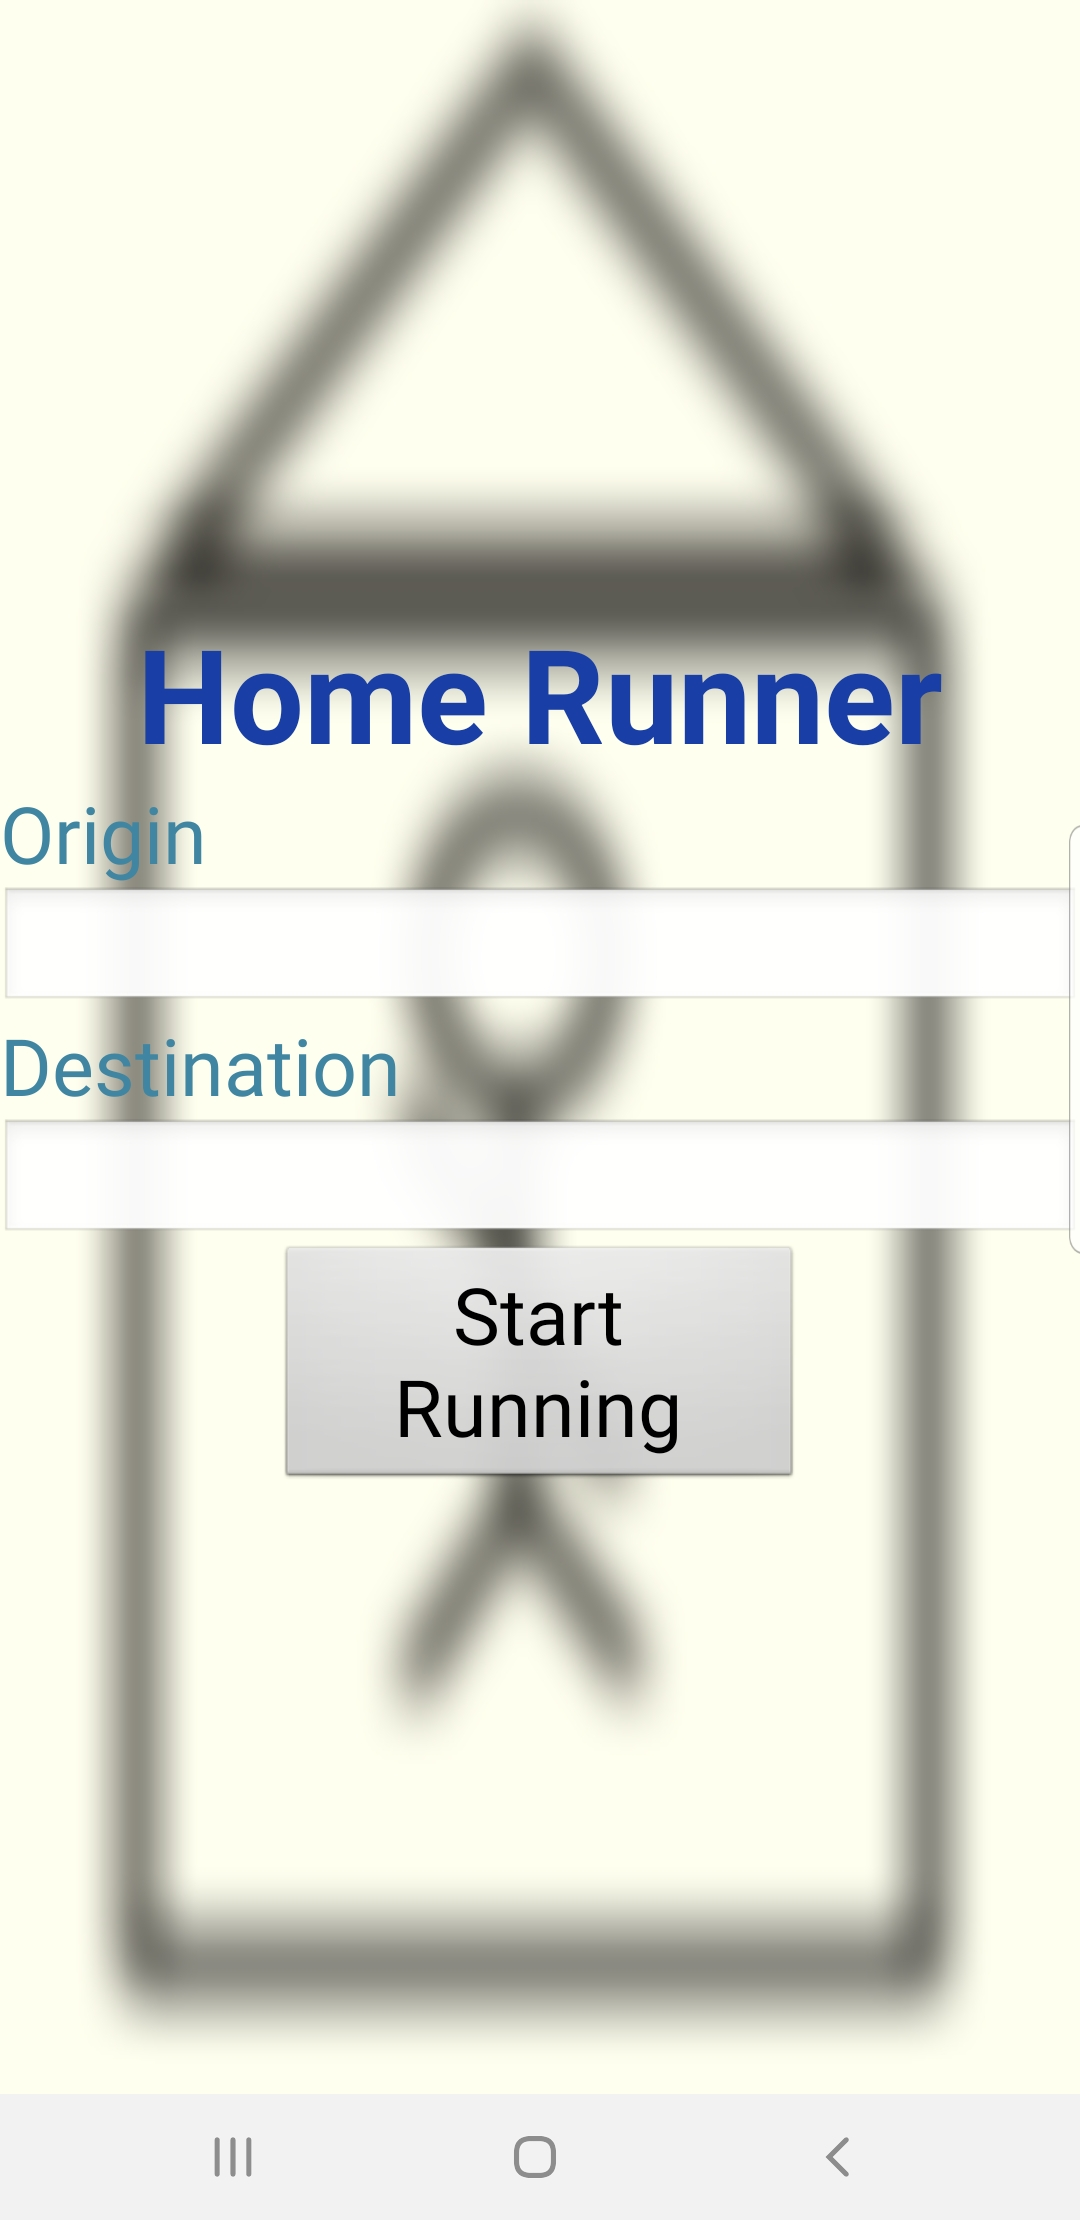
\includegraphics[scale=0.3]{Gambar/main-page.png}
	\caption{Halaman utama aplikasi}
	\label{fig:main-page}
\end{figure}

\subsubsection{\textit{Textbox}} 
\textit{Textbox} adalah komponen pada antarmuka yang menerima masukan pengguna yang berupa tulisan atau \textit{string}. Ada dua buah \textit{textbox} pada halaman utama ini. \textit{Textbox} pertama akan menerima masukan pengguna yang merupakan lokasi asal dari rute lari, dan \textit{textbox} kedua akan menerima masukan berupa lokasi tujuan dari rute lari yang diinginkan pengguna.   

\subsubsection{Tombol ``\textit{Start Running}''}
Tombol "\textit{Start Running}" adalah tombol yang akan memicu halaman VR yang sesuai dengan informasi dari dua \textit{textbox} di atas ketika ditekan. Tombol ini berada di bawah \textit{destination textbox}.

\subsection{Halaman VR}
Halaman VR adalah halaman yang menampilkan pemandangan VR secara VR ketika berlari. Untuk memunculkan halaman ini, pengguna harus menekan tombol dari halaman utama (dijelaskan pada Subbab \ref{subs:main-page}) terlebih dahulu. Karena posisi gawai masih dalam keadaan \textit{portrait}, ada satu halaman terlebih dahulu yang muncul seperti di Gambar \ref{fig:cardboard-page}. 

\begin{figure}[h]
	\centering
		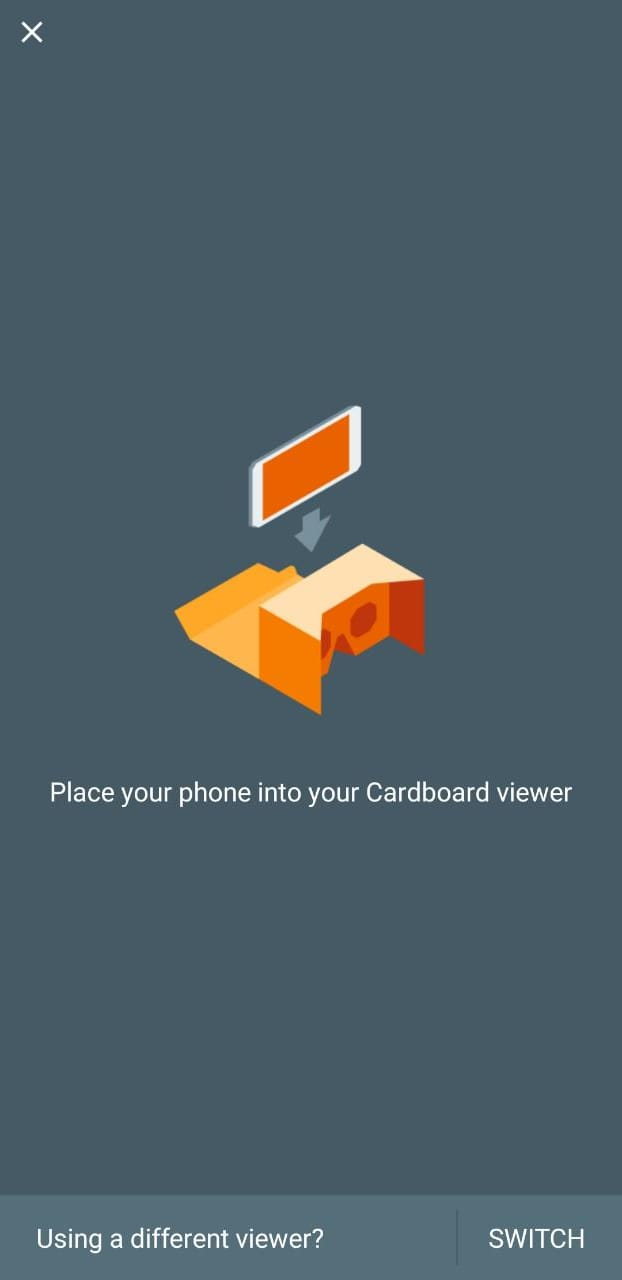
\includegraphics[scale=0.4]{Gambar/cardboard-page.png}
	\caption{Halaman \textit{Google Cardboard} sebelum gawai diputar}
	\label{fig:cardboard-page}
\end{figure}

Halaman ini dimunculkan ketika mengakses \textit{Google Cardboard}. Untuk menuju ke halaman VR, pengguna harus memutar gawai sehingga gawai berada dalam posisi \textit{landscape}. Setelah gawai berada dalam posisi \textit{landscape}, halaman VR akan dimunculkan seperti yang ditunjukkan pada Gambar \ref{fig:vr-page}.

\begin{figure}[h]
	\centering
		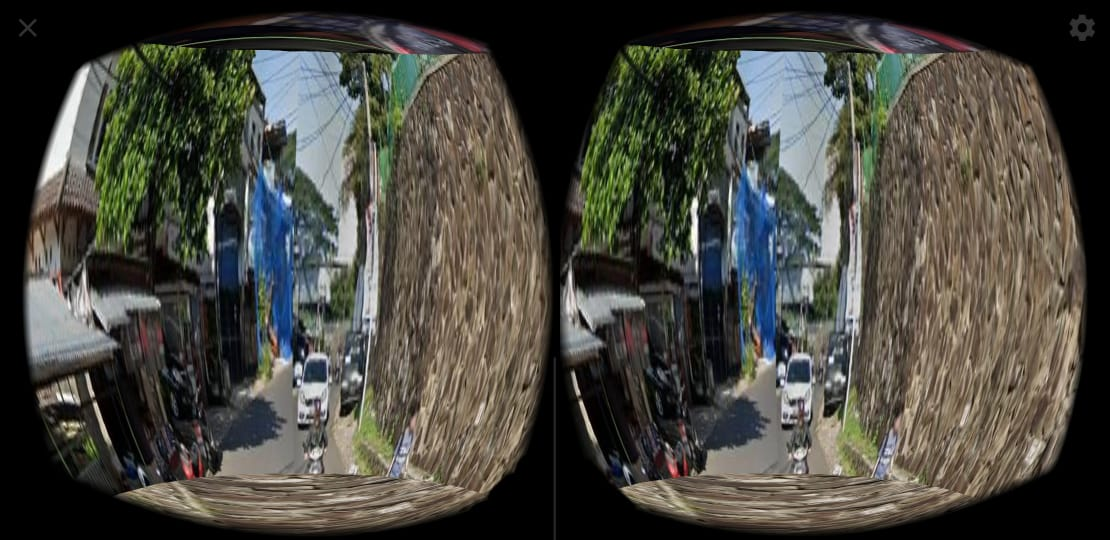
\includegraphics[scale=0.4]{Gambar/vr-page.png}
	\caption{Halaman VR dari aplikasi}
	\label{fig:vr-page}
\end{figure}

Pada tampilan VR tersebut, gambar akan berubah-ubah sesuai dengan langkah kaki pengguna. Perubahan tersebut akan terjadi ketika mencapai pengguna mencapai jarak 100 meter. Jika pengguna sudah mencapai tujuan sesuai dengan jarak yang ditempuh, halaman VR akan berhenti mengubah gambar.     

\section{Rancangan Program}
Subbab ini akan menjelaskan rancangan  program, mulai dari rancangan kelas dan algoritma-algoritma yang digunakan pada \textit{method-method} yang penting. 

\subsection{Rancangan Kelas}
Rancangan kelas dari aplikasi akan menggunakan seluruh bagian pada aplikasi HelloVR dan beberapa tambahan kelas. Gambar \ref{fig:class-diagram} menunjukkan atribut-atribut dan \textit{method-method} dari masing-masing kelas, serta hubungan antara satu kelas dan kelas-kelas lain. 

\begin{figure}[h]
	\centering
		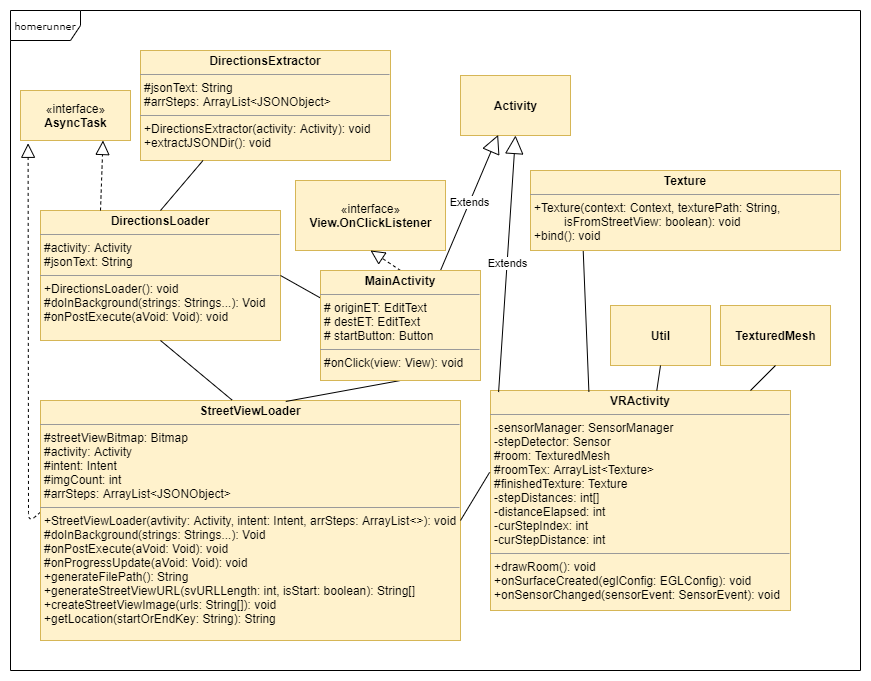
\includegraphics[scale=1]{Gambar/class-diagram.png}
	\caption{Diagram \textit{class} dari Aplikasi}
	\label{fig:class-diagram}
\end{figure}

Beberapa kelas di Gambar \ref{fig:class-diagram} tidak memiliki deskripsi lebih karena berasal dari \textit{library} Java ataupun \textit{Google VR SDK}. Kelas-kelas yang ditambahkan adalah:

%Lengkapi penjelasan
\begin{enumerate}
	\item \texttt{MainActivity}
	
	Kelas yang mengelola halaman utama. Atribut yang dimiliki kelas ini:
	
	\begin{itemize}
		\item \texttt{protected EditText originET}
		
		Bagian dari antarmuka yang dapat menerima masukan lokasi asal dari rute lari.
		\item \texttt{protected EditText destET}
		
		Bagian antarmuka yang dapat menerima masukan lokasi tujuan dari rute lari.
		\item \texttt{protected Button startButton}
		
		Tombol yang digunakan untuk memicu halaman VR.
		\item \texttt{protected StreetViewLoader streetViewLoader}
		
		Atribut dari \textit{loader} gambar \textit{StreetView} untuk inisialisasi di halaman VR.
	\end{itemize}
	
	\textit{Method-method} yang dimiliki kelas ini adalah:
	
	\begin{enumerate}
		\item \texttt{protected void onClick(View view)}
		
		\textit{Method} yang dijalankan ketika komponen yang sudah dipasangkan \texttt{onClickListener} ditekan. 
		\item \texttt{public String[] generate StreetView()}
		
	\end{enumerate}
	\item \texttt{HelloVRActivity}
	
	Kelas yang mengelola halaman VR.
	\item \texttt{StreetViewLoader}
	
	Kelas yang berfungsi untuk memuat gambar \textit{StreetView} dan menyatukan semua gambar itu, membentuk gambar pemandangan yang utuh.  
	\item \texttt{DirectionsLoader}
	
	Kelas yang memuat JSON dari rute lari. 
\end{enumerate} 


\subsection{Algoritma-Algoritma yang digunakan}
Ada beberapa algoritma yang digunakan   untuk melakukan beberapa proses seperti mengolah \textit{Google StreetView API},\textit{Google Directions API}, dan menampilkan .

\subsubsection{Mengolah \textit{Google StreetView API}} 
\textit{StreetView API} berfungsi untuk memuat gambar pemandangan dan menggunakan menggunakan HTTP/HTTPS. Karena sekali pemanggilan hanya menghasilkan gambar dari satu arah pemandangan, empat gambar dari empat pandangan haruslah diunduh terlebih dahulu. Setelah semua gambar itu terunduh, semua gambar itu disatukan, menjadi satu gambar untuk menjadi tekstur bangun ruang silinder. Algoritma yang digunakan untuk menyatukan gambar-gambar tersebut. Setelah gambar-gambar itu sudah disatukan, gambar tersebut harus disimpan di dalam \textit{file} pada \textit{StreetView} tersebut adalah: Langkah-langkah untuk memuat dan mengolah gambar-gambar untuk menyajikan gambar pemandangan yang utaha adalah:

	\begin{enumerate}
		\item Memuat gambar \textit{StreetView} dari semua arah lewat HTTP/HTTPS. 
		
		\item Menggabungkan gambar  \textit{StreetView} dari semua arah yang sudah dimuat.
		
		\item Menyimpan gambar dalam \textit{cache}.
	\end{enumerate}
	
Setelah gambar yang sudah disatukan dan disimpan dalam \textit{file} di \textit{cache}, barulah gambar itu bisa digunakan sesuai kebutuhan.


\subsubsection{Mengolah \textit{Google Directions API}}
\textit{Directions API} adalah \textit{API} yang menggunakan protokol HTTP/HTTPS dan menghasilkan keluaran dalam bentuk JSON. Untuk memuat JSON berisi rute perjalanan dari asal sampai tujuan, pemanggilan \textit{Directions API} harus dilakukan melalui HTTP/HTTPS. Setelah  JSON dari rute lari diperoleh dari \textit{Directions API}, JSON rute disimpan di \textit{cache} perangkat pengguna.

Setelah JSON disimpan dalam \textit{file}, JSON rute lari dapat digunakan dengan membaca atribut dan nilai-nilainya sesuai kebutuhan. Beberapa nilai atribut dalam JSON ini  berupa JSON \textit{object}, ada yang berupa JSON \textit{array}. Karena hal ini,  \textit{parsing} dari JSON ini harus dilakukan sesuai dengan ketentuan tersebut. 


%\section{\textit{Folder Assets}}
%
%\textit{Folder assets} mengandung \textit{asset-asset} multimedia seperti gambar dan \textit{audio}. 
%Menghapus \textit{file-file} dari aplikasi HelloVR. 
%
%Mengganti CubeRoom.obj dengan file OBJ dengan bangun ruang silinder.
%
%Mengganti file CubeRoom\_BakedDiffuse.png, menggantinya dengan gambar \textit{StreetView} yang sudah disatukan. 


